% !TeX root = ../thuthesis-example.tex

\chapter{仿真平台搭建及分析}

\section{本章引言}

本章介绍仿真平台的搭建,并对仿真平台的真实性进行分析。仿真平台中的车辆是根据其跟驰策略行驶的,在本章中将首要介绍人工驾驶车辆和自动驾驶车辆选用
的跟驰模型;接着将简要介绍仿真所用的平台以及仿真的参数;最后,由于仿真的真实性将直接影响本工作的实际意义,所以在本章中将会对仿真的真实性进行分析。

本章的结构如图\ref{fig:chap02-1-logic}所示。

\begin{figure}
  \centering
  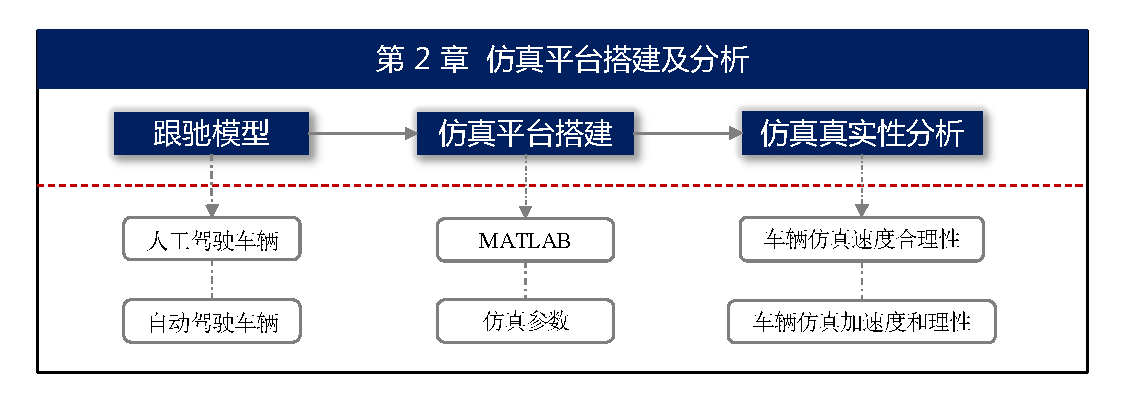
\includegraphics[width=1\linewidth]{chap02-1-structure.pdf}
  \caption{第2章结构}
  \label{fig:chap02-1-logic}
\end{figure}

\section{跟驰行为建模}

在本课题中,需要对人工驾驶和自动驾驶两种车辆的跟驰行为建模。

\subsection{人工驾驶车辆跟驰模型}

根据第一章中对跟驰行为建模研究现状的综述,对于人工驾驶车辆选择表达形式直观,参数量适中,对实际情况拟合情况较好的速度优化跟驰模型(OVM)。其具体表达式为

\begin{align}
  \dot{v}_n(t) &= \kappa \left\{ V \left[ h_n(t) \right] - v_n(t) \right\} \notag \\
  V \left[ h_n(t) \right] &= v_0 \left\{ 1 - \exp \left[ - \frac{\alpha}{v_0}\left(h_n(t)-s_0\right) \right] \right\}
  \label{eq:chap02-1}
\end{align}
其中,各符号含义在表\ref{tab:chap01-5}中给出,其相关参数取值如表\ref{tab:chap01-2}所示。

\begin{table}
  \centering
  \caption{速度优化跟驰模型参数取值}
  \begin{tabular}{cc}
    \toprule
    参数          &  取值                         \\
    \midrule
    敏感系数$\alpha$        & $0.999s^{-1}$         \\
    敏感系数$\kappa$       & $0.700s^{-1}$             \\
    自由流速度$v_0$             & $33.0 m/s$          \\
    最小安全距离$s_0$             & $1.62m$        \\
    \bottomrule
  \end{tabular}
  \label{tab:chap02-1}
\end{table}

下面对该跟驰模型进行简要分析。

速度优化函数描述了在当前车与前车的车头间距给定后,当前车驾驶员存在一个希望保持的理想的速度。图\ref{fig:chap02-2-OVM1}描述了这个理想速度的大小与两车车头距离的关系。
可以观察到速度优化函数在其定义域内是单调递增的,即前车距离越远,驾驶员希望保持的理想速度越大,以尽快缩小与前车的距离;当前车距离越近,驾驶员希望保持的理想速度越小,以减小
追尾的风险,这与真实情况是一致的。

\begin{figure}
  \centering
  \subcaptionbox{OVM速度优化函数图像\label{fig:chap02-2-OVM1}}
    {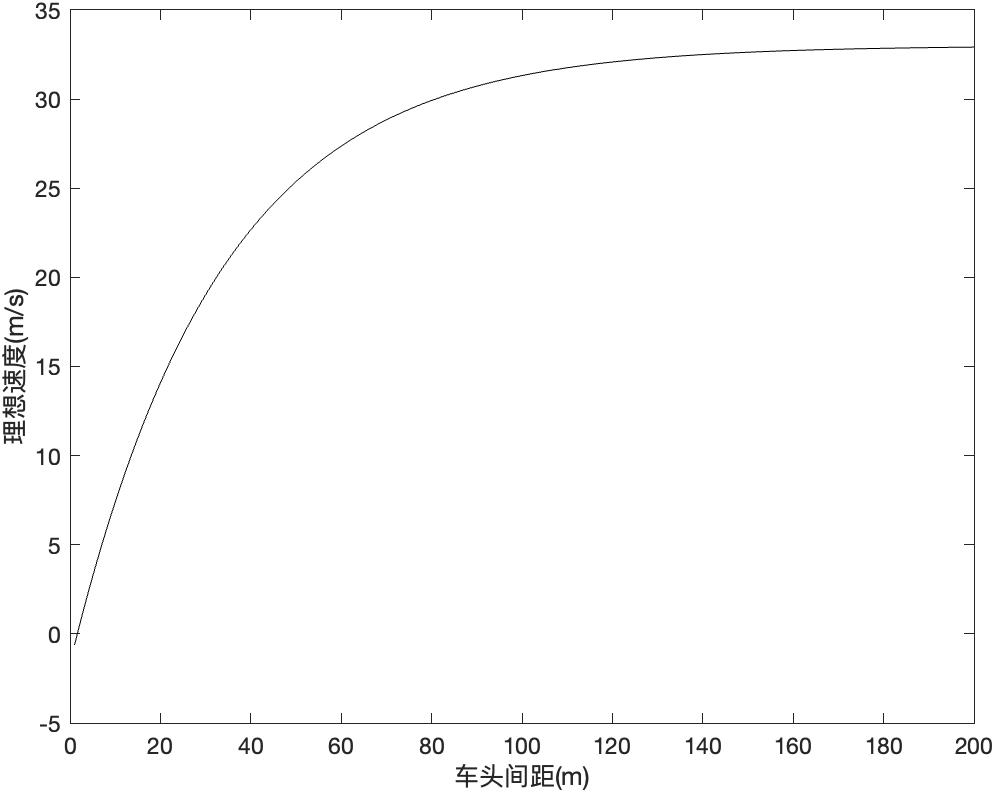
\includegraphics[width=0.45\linewidth]{chap02-2-OVM1.jpg}}
  \subcaptionbox{加速度与当前速度、车头间距的关系\label{fig:chap02-2-OVM2}}
    {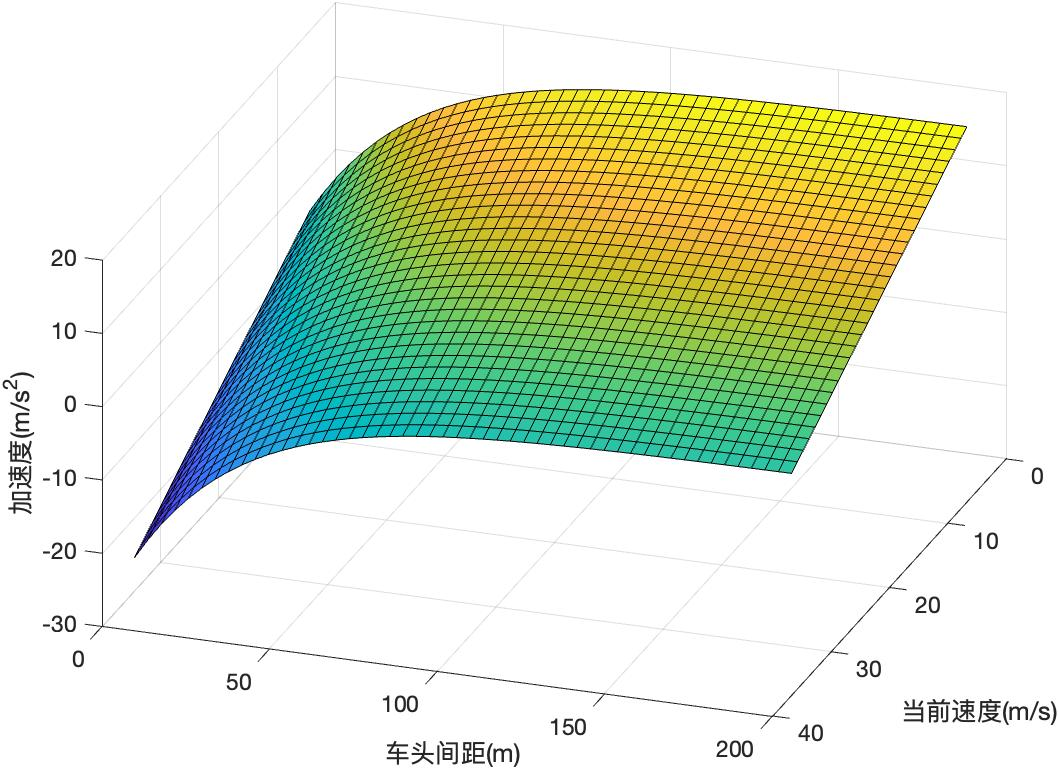
\includegraphics[width=0.5\linewidth]{chap02-2-OVM2.jpg}}
  \caption{OVM函数关系图像}
  \label{fig:chap02-2-OVM}
\end{figure}

图\ref{fig:chap02-2-OVM2}描述了车头时距、当前速度、加速度三者的关系。可以观察到当当前速度固定时,车头时距越大,加速度也越大,且呈现出与速度优化函数一样的增长规律,这与
式\ref{eq:chap02-1}是相符合的;当车头间距固定时,理想速度也就确定了,所以随着当前速度的增大,加速度线性减小。

\subsection{自动驾驶车辆跟驰模型}

自动驾驶车辆选择基于PID控制的车头时距控制算法来控制跟驰行为,该算法的表达式见式(\ref{eq:chap02-2})。
\begin{equation}
  \dot{v}_n(t) = k_1 \left[ h_n(t) - l - t_hv_n(t) \right] + k_2 \left[ v_{n-1}(t) - v_n(t) \right]
  \label{eq:chap02-2}
\end{equation}
其中,各符号含义在表\ref{tab:chap02-2}中给出

\begin{table}
  \centering
  \caption{基于PID控制的车头时距控制算法符号说明}
  \begin{tabular}{cc}
    \toprule
    符号          &  含义                         \\
    \midrule
    $k_1, k_2$            & 控制步长         \\
    $t_h$                 & 理想车头时距             \\
    $l$                   & 车身长度          \\
    $h_n(t)$              & 第$n$辆车在$t$时刻与前车的车头间距        \\
    $v_n(t)$              & 第$n$辆车在$t$时刻的速度 \\
    \bottomrule
  \end{tabular}
  \label{tab:chap02-2}
\end{table}

可以发现在该算法控制下,车辆的加减速由两部分控制。一是当前的两车车头距离与理想的车头距离的大小关系,如果当前两车车头距离小于理想的车头距离,那么参数$k_1$控制的部分倾向于减速;
二是当前车与前车的速度大小关系,如果当前车速度大于前车速度,$k_2$控制的部分倾向于减速。通过改变$k_1$和$k_2$的值,可以调节这两个部分的权重,二者综合即可决定当前车应当加速还是
减速,以及加速度的大小。


\section{仿真平台的搭建}

仿真基于MATLAB软件,模拟了一个由11辆车组成的车队,如图\ref{fig:chap02-3-simu1}所示。车队中的第一辆车是头车,其既不是人工驾驶车辆也不是自动驾驶车辆,而是按照实现规定好的策略行驶,即在0时刻以$-2m/s^2$的
加速度减速到原速度的$90\%$,紧接着以$2m/s^2$的加速度恢复元素,其速度变化情况如图\ref{fig:chap02-3-simu2}所示。如此设置头车是为了加入扰动,虽扰在真实场景下扰动可能发生在车队中的任何一辆车上,由于受到
该扰动影响的车辆是此车之后的车辆,只要将此车看作头车,就与仿真实验场景一致了,所以这样的仿真情景具有一定的一般性。

\begin{figure}
  \centering
  \subcaptionbox{车队示意图\label{fig:chap02-3-simu1}}
    {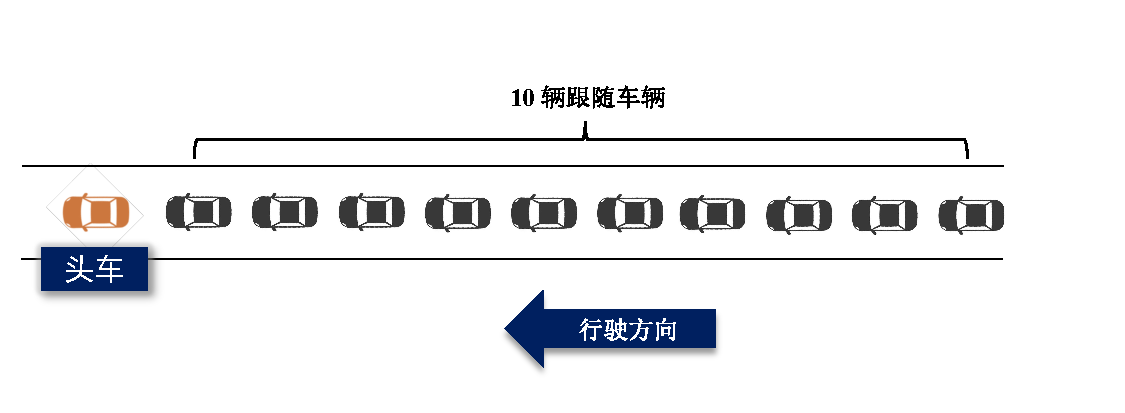
\includegraphics[width=1\linewidth]{chap02-3-simu1.pdf}}
  \subcaptionbox{头车速度变化曲线(初速度$20m/s$,截取前$10s$)\label{fig:chap02-3-simu2}}
    {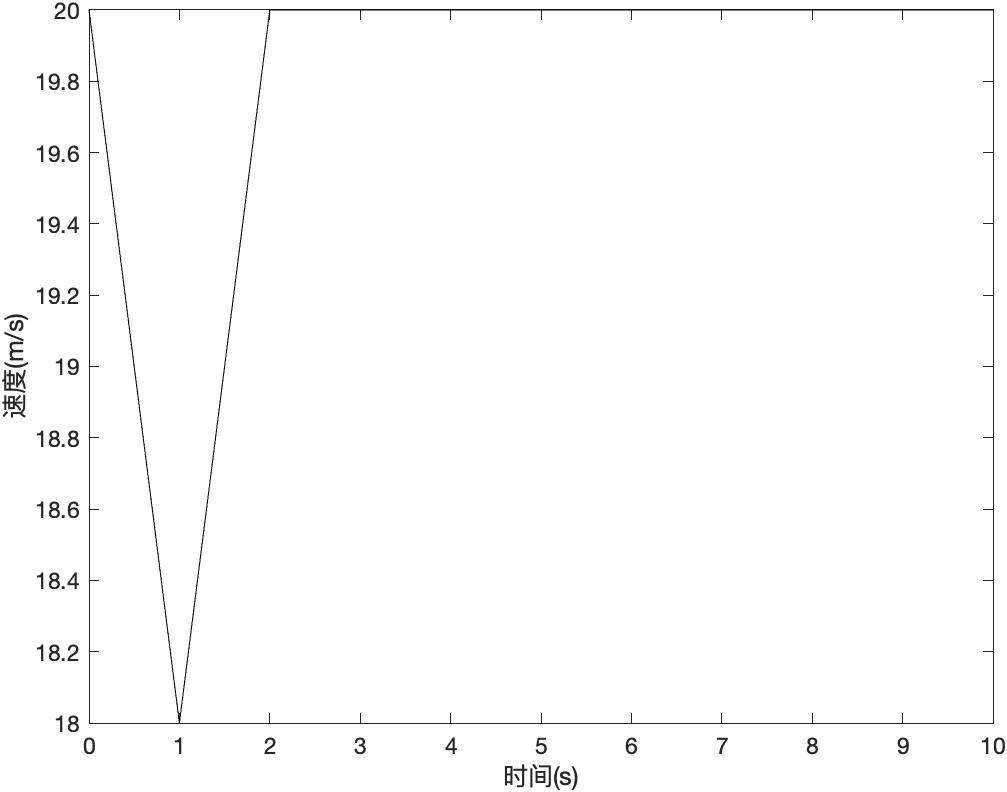
\includegraphics[width=0.6\linewidth]{chap02-3-simu2.jpg}}
  \caption{仿真场景设置}
  \label{fig:chap02-2-simu}
\end{figure}

为了数值仿真只能模拟,首先将连续场景离散化。为了尽量减小误差,仿真步长取$0.01s$,总仿真时长为$500s$,这意味着有50000个采样点。

为了使仿真尽可能的接近真实情况,也应考虑实际情况中的物理限制,如真实场景下车辆的加速度大小是限制在一定范围内的,这由轮胎与道路摩擦因数等原因决定。


\section{仿真平台真实性分析}

